\chapter{Vista de implementación}

\section{Introducción}
Esta seccion describe la estructura general de la implementaicon del sistema. Muesta la descomposicion del sistema en subsistemas y cuales de estos son los mas importantes. Comprende a grandes rasgos todos aquellos artefactos que se utilizan para ensamblar el sistema y ponerlo en producción, ya listo para su distribución física

La arquitectura del sistema esta distribuida en 3 capas
\begin{enumerate}
\item Presentaci\'on: Esta constituida por todos aquellos componentes visibles para el usuario junto con pequeños submodulos de validacion de datos de entrada y salida. Los usuarios, podrán acceder a esta capa de presentación a través de las siguientes plataformas:
\begin{enumerate}
\item Web: podr\'an acceder a trav\'es de cualquier ordenador con conexi\'on local (si se encuentra en el entorno EHC) o por Internet.
\item M\'ovil: dispondr\'an tanto de una aplicaci\'on para iOS como para Android. A través de esta plataforma también es posible conectarse via local o via Internet.
\end{enumerate}
\item Aplicaci\'on: en esta capa englobamos todo aquello a la l\'ogica de la aplicaci\'on, además de proveer toda la lógica funcional para conectar la capa de presentación con la capa de transferencia de datos . 
\item Datos:   Esta capa consiste en una base de datos MYSQL que provee persistencia de datos. Se sirve de "procedimientos almacenados" que poseen acceso directo a los propipos datos de la base de datos con lo que se consigue fluidez y buena respuesta en la base de datos
    Esta capa se comunica con la capa de Servicio Web para responder a las peticions SQL.
\end{enumerate}


\section{Vista general del sistema}

La arquitectura del sistema está definida en la figura ~\ref{fig:arquitectura}. En dicha figura, podemos destacar los siguientes elementos y características:
\begin{itemize}
\item Dispositivo: el acceso al sistema EHC se puede realizar mediante:
\begin{itemize}
\item Dispositivo móvil: usando las aplicaciones disponibles tanto para iOS como para Android.
\item Ordenador: a través del portal EHC.
\end{itemize}
\item Servidor: será el encargado de enviar las peticiones del usuario a desde el dispositivo origen al entorno EHC a través de Internet. También será el encargado de almacenar toda la información requerida para el sistema.
\item Router: será necesario para poder almacenar la información del entorno EHC y para poder enviar/recibir peticiones a través de Internet.
\item Raspberry PI: funcionará como servidor local del entorno EHC. Será el encargado de gestionar las peticiones recibidas a través de la red local y/o de Internet hacia los dispositivos domotizados del hogar.
\item Arduino: es el subsistema encargado de controlar todos los sensores y actuadores instalados en un dispositivo.
\item Envio de peticiones: como ya se ha mencionado, estas peticiones pueden realizarse a través de Internet o a través de una red local donde estén conectados tanto el terminal origen como el servidor local.
\end{itemize}

\begin{figure}[h!]
	\centering
	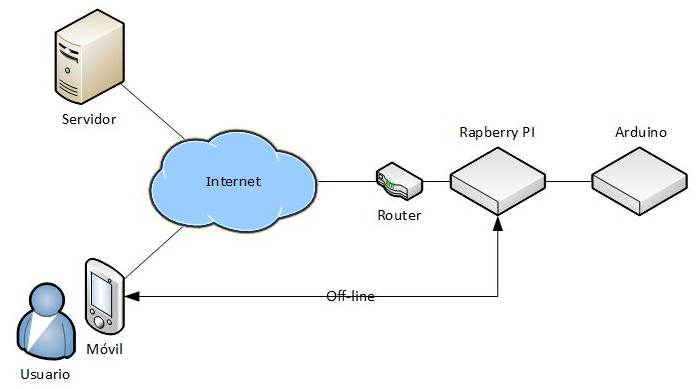
\includegraphics[width=0.8\textwidth]{4.Disenio/Imagenes/arquitectura}
	\caption{Arquitectura del sistema.}
	\label{fig:arquitectura}
\end{figure}


%%%%%%%%%%%%%%%%%%%%%%%%%%%%%%%%%%%%%%%%%%%%%%%%%%%%%%%%%%%%%%%%%%%%%%%%%%%%%%%%%%%
